The Back Burner Brew system will consist of five different subsystems: brew
system vessels, analog components, digital components, web server, and the user
interface. The brew system vessels will be operated through the analog
components. The analog components will send data to digital components. The
analog components will be controlled by the digital components based on what is
input to the user interface or certain conditions that are predefined such as
keep water a certain temperature. The web server will be the intermediary
between the user interface and the digital components. The web server will also
store all data associated with the brewing process such as temperature or time
spent on specific tasks.

\begin{figure}[H]
	\centering
	\graphicspath{.\images}
	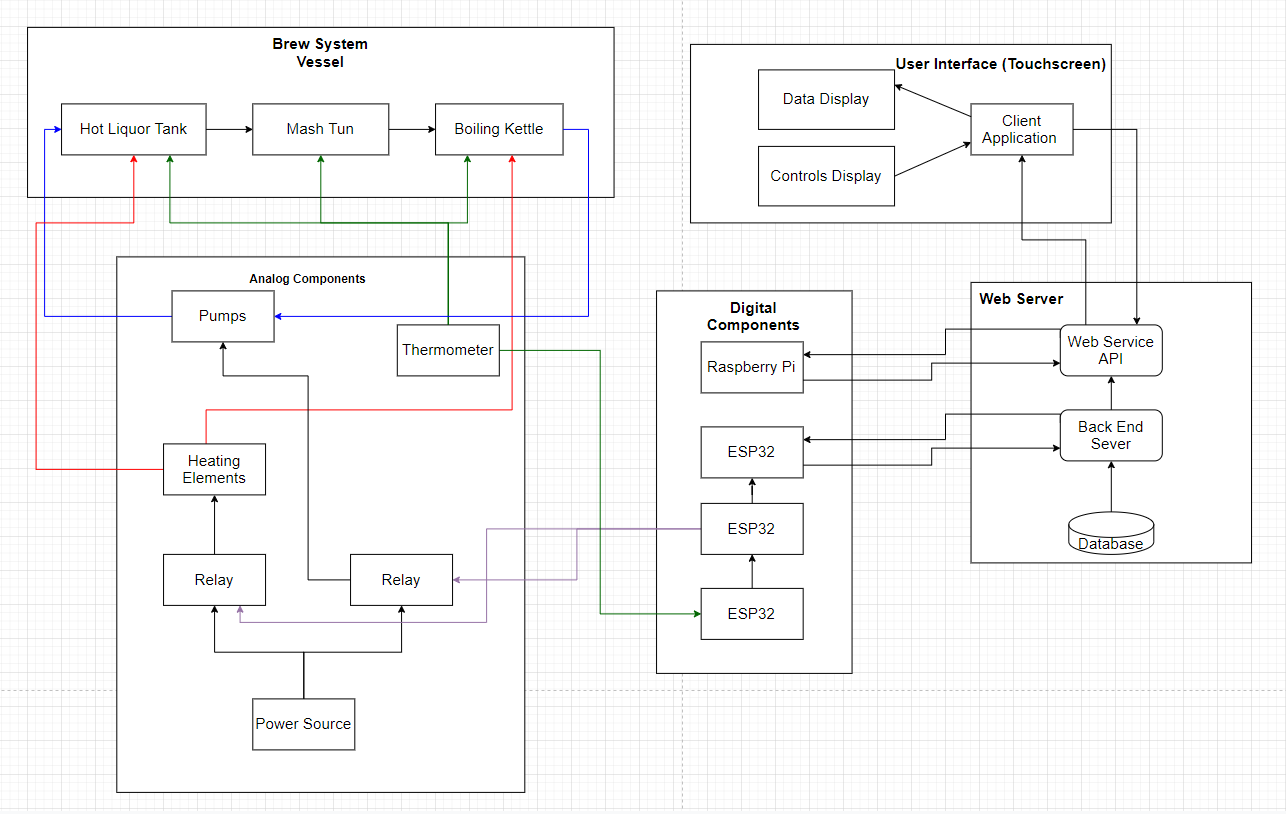
\includegraphics[scale=0.5]{images/ADS_system.PNG}
	\caption{Subsystem Diagram for the Back Burner Brew device.}
\end{figure}